\lab{Application}{Cracking Blackjack}{Cracking Blackjack}
\label{Ch:BJ}

\objective{Exploit the weaknesses of a pseudorandom number generator that is based on a Linear Congruential Generator.}

\section*{Blackjack}

\begin{figure}[H]
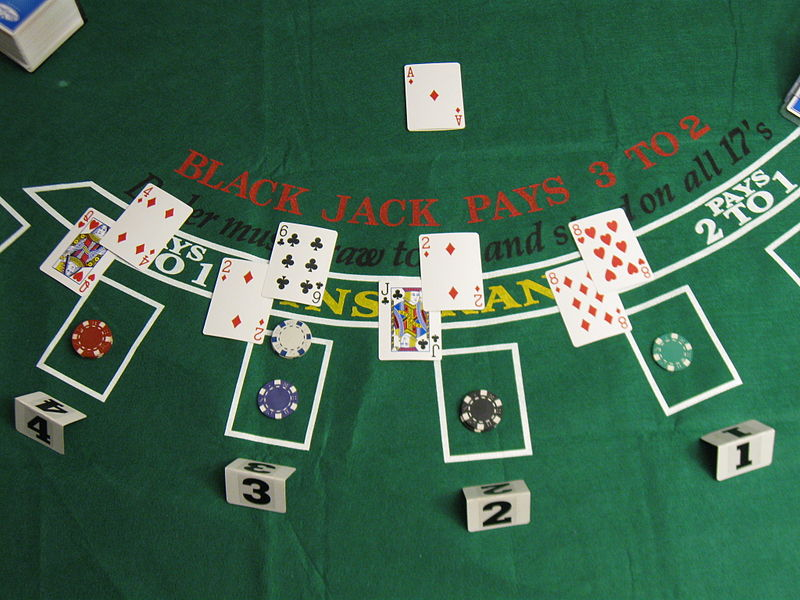
\includegraphics[scale = .9]{Blackjack_game_1.jpg}
\caption{Initial Round of a BlackJack Game}
\end{figure}

Black Jack is a card game that involves the use of randomness.
The game is simple.
The dealer deals the player and himself each two cards.
He flips over his first card so that the player can see it.
The player has to choose to take another card ("hit") or not ("stand").
If the player hits he gets another card and again has the choice to hit or stand.

The goal is to get your hand to be at or as close to 21 without going over.
Face cards are worth 10 points.
Aces can count either as 11 or 1.
The value of all other cards are equal to number on the card.

Once the player has decided to stand the dealer flips over his second card and deals himself cards until his hand value is 17 or greater. 

If the player value goes above 21 he automatically loses.
If his value is 21 and below and dealer has above 21 then the player wins.
If they both have 21 or under than the player with the hand of highest value wins.
If both hands have the same value, the game is a tie.

\section*{Shuffling Algorithms}

One use of Pseudorandom Number Generators (PRNGs) is to shuffle cards.
The main goal of these algorithms is that the card order be random--so that no single player has an advantage based on order.
Often, as strange as it may seem, online gambling sites will post their shuffling algorithms online.
The only things they do not post are their seed values.
Often the time in milliseconds from midnight is used as the seed value.

John von Neumann said ``Anyone who considers arithmetical methods of producing random digits is, of course, in a state of sin."
As seen in the last lab, weak PRNGs are periodic and are predictable once a few outputs are known.
This lab will have you break blackjack based on a weak PRNG.

\section*{Cracking Blackjack}
For these next problems you will need three files that are provided with this lab: Black.py, BlackEasy.py, and bjHelp.py.
Black.py and BlackEasy.py are are programs that run games of Blackjack that use a Linear Congruentail Generator (LCG) to shuffle the cards.
They generate 52 random numbers and then the argsort of those numbers is the order of the cards.
The parameters for BlackEasy.py are a$=2521$, c$=13$, mod$=2^{16}$.
For Black.py they are a$=25214903917$, c$=11$, mod$=2^{48}$.
In order to play them type \li{python <<filename>> <<numberofgames>>} in your command line.
They are both seeded initially by the time.

bjHelp.py contains two functions that will help you "predict" the cards:
SuffleHack(n,a,c,mod,seed) gives the first $n$ card shuffles given the parameters for a LCG.
The shuffles are represented by numbers.
Hacker(Stats,['card','card','card']) Stats is the output of SuffleHack and takes a list of 3 cards (see below).
It prints all shuffles as a list of cards in Stats that have the same first three cards as the inputted list.

The trick to being able to "predict" the cards is to find the initial seed value.

Cards- A, 2-10, J, Q, or K combined with heart, diamond, club, or spade in single quotes.
Examples: '6diamond', 'Kclub'.

\begin{warn}
Both BlackEasy.py and Black.py use functions that are incompatible with ipython. They need to run \li{python Black.py} in command line.
\end{warn}



\begin{problem}
Play 10 games of BlackEasy.py and by the 5th game be able to predict the cards.
You can write your own functions or use the ones in bjHelp.py.
You will want to open two command prompts, one to play the game and one to predict the cards. 
\end{problem}

Not too hard.
That is because there is only $2^{16}$ seed values.
This next one you will have to look at more hands until you can find out the initial seed value.

\begin{problem}
Play 20 games of Black.py and by the 15th game be able to predict the cards.
\end{problem}



